\documentclass[11pt,a4paper]{article}

% ── Packages ──────────────────────────────────────────────────────────────────
\usepackage[a4paper, margin=1in]{geometry}
\usepackage[utf8]{inputenc}
\usepackage[T1]{fontenc}
\usepackage{lmodern}
\usepackage{microtype}
\usepackage{setspace}
\usepackage{titlesec}
\usepackage{titling}
\usepackage{fancyhdr}
\PassOptionsToPackage{hyphens}{url}
\usepackage[hidelinks]{hyperref}
\usepackage{xcolor}
\usepackage{booktabs}
\usepackage{array}
\usepackage{longtable}
\usepackage{enumitem}
\usepackage{parskip}
\usepackage{graphicx}
\usepackage{amsmath}
\usepackage{amssymb}
\usepackage{caption}
\usepackage{tabularx}
\usepackage{multirow}
\usepackage{colortbl}
\usepackage{tcolorbox}
\usepackage{listings}

% ── Neutral academic palette (no bright colour on body text or tables) ───────
\definecolor{ink}{RGB}{26, 26, 26}
\definecolor{subink}{RGB}{60, 60, 60}
\definecolor{darkgray}{RGB}{90, 90, 90}
\definecolor{medgray}{RGB}{170, 170, 170}
\definecolor{lightgray}{RGB}{245, 245, 245}
\definecolor{headerbg}{RGB}{55, 62, 74}
\definecolor{headertext}{RGB}{255, 255, 255}
\definecolor{rowalt}{RGB}{244, 246, 248}
\definecolor{accent}{RGB}{74, 85, 104}
\definecolor{donegray}{RGB}{60, 60, 60}
\definecolor{proggray}{RGB}{120, 120, 120}
\definecolor{pendinggray}{RGB}{170, 170, 170}

% Compatibility aliases (table bodies reference these names)
\colorlet{acmblue}{ink}
\colorlet{rowblue}{headerbg}

% ── Hyperref setup ────────────────────────────────────────────────────────────
\hypersetup{
    colorlinks=true,
    linkcolor=accent,
    citecolor=accent,
    urlcolor=accent,
    pdftitle={Final Project Report: Auditing Geographic and Cultural Bias in Clinical LLMs},
    pdfauthor={Group 7 - LUMS CS-5312 Spring 2026},
}

% ── Section formatting (neutral ink, no accent colour) ────────────────────────
\titleformat{\section}
  {\large\bfseries\color{ink}}
  {\thesection}{1em}{}
  [\vspace{-4pt}\rule{\linewidth}{0.6pt}\vspace{2pt}]

\titleformat{\subsection}
  {\normalsize\bfseries\color{ink}}
  {\thesubsection}{1em}{}

\titleformat{\subsubsection}
  {\normalsize\bfseries\itshape\color{subink}}
  {\thesubsubsection}{1em}{}

% ── Float placement: keep tables/figures near their reference without
%     forcing half-empty pages. ─────────────────────────────────────────────
\renewcommand{\topfraction}{0.9}
\renewcommand{\bottomfraction}{0.8}
\renewcommand{\textfraction}{0.08}
\renewcommand{\floatpagefraction}{0.75}
\setcounter{topnumber}{3}
\setcounter{bottomnumber}{3}
\setcounter{totalnumber}{5}

% ── Discourage widow/orphan lines; allow natural page bottoms ────────────────
\widowpenalty=10000
\clubpenalty=10000
\raggedbottom

% ── Header / Footer ───────────────────────────────────────────────────────────
\pagestyle{fancy}
\fancyhf{}
\fancyhead[L]{\small\textcolor{darkgray}{Final Project Report}}
\fancyhead[R]{\small\textcolor{darkgray}{Big Data Analytics (CS 5312)}}
\fancyfoot[C]{\small Page \thepage}
\renewcommand{\headrulewidth}{0.4pt}
\renewcommand{\footrulewidth}{0pt}

\setstretch{1.15}
\setlist[itemize]{leftmargin=1.5em, itemsep=3pt, topsep=4pt}
\setlist[enumerate]{leftmargin=1.5em, itemsep=3pt, topsep=4pt}

% ── Line-breaking leniency so long paths / table rows never overflow ─────────
\setlength{\emergencystretch}{3em}
\sloppy

% ── Breakable code-path macro ─────────────────────────────────────────────────
\usepackage{url}
\urlstyle{tt}
\makeatletter
\g@addto@macro\UrlBreaks{\do\_\do\-\do\.}
\makeatother
\newcommand{\pathtt}[1]{\mbox{}\nolinkurl{#1}}

% ── Listings setup for code snippets ──────────────────────────────────────────
\lstset{
  basicstyle=\ttfamily\footnotesize,
  commentstyle=\color{darkgray}\itshape,
  keywordstyle=\color{ink}\bfseries,
  stringstyle=\color{subink}\itshape,
  frame=single,
  framerule=0.4pt,
  rulecolor=\color{medgray},
  backgroundcolor=\color{lightgray},
  breaklines=true,
  columns=fullflexible,
  showstringspaces=false,
  captionpos=b,
  xleftmargin=6pt,
  xrightmargin=6pt,
}

% ═══════════════════════════════════════════════════════════════════════════════
\begin{document}

\graphicspath{{figs/}}

% ── Title Block ───────────────────────────────────────────────────────────────
\begin{center}
{\Large\textbf{Final Project Report:\\[0.2em]
Auditing Geographic and Cultural Bias in Clinical Large Language Models}}\\[1.0em]

\textbf{Group 7 Members:}\\[0.3em]
Taimour Abdul Karim (24280047)\\
Syed Muhammad Mujtaba (24280069)\\
Usmar Haider (24280052)\\
Shawal Latif (24280068)\\
Abdul Moeed Irshad (24280046)\\[0.8em]

\textbf{Course:} Big Data Analytics (CS 5312)\qquad\textbf{Semester:} Spring 2026\\
\textbf{Instructor:} Dr.\ Imdadullah Khan\qquad\textbf{Institution:} Lahore University of Management Sciences (LUMS)\\
\textbf{Submission Date:} May 18, 2026
\end{center}

\vspace{0.8em}\hrule\vspace{0.8em}

% ── Abstract ──────────────────────────────────────────────────────────────────
\begin{abstract}
\noindent This is the final report of a project that audits geographic and
cultural bias in clinical large language models (LLMs). It builds on the
intermediate report and extends Gourabathina et~al.~\cite{gourabathina2025}
along an axis that prior work has not studied: whether a patient who reads as
Global~South rather than Global~North gets systematically different clinical
recommendations from an LLM when every clinical fact is held fixed. We built a
reproducible, stdlib-only five-stage audit pipeline that handles dataset and
Name-Bank construction, deterministic perturbation, multi-provider inference
over OpenAI, Groq, and AWS~Bedrock, LLM-based annotation, and statistical
analysis. From that pipeline we compute a Geographic Disparity Index (GDI),
derived from a Reduced-Care-Errors Rate (RCER) on a matched-pair design. Three
experiments were run end-to-end and are reported in full. \emph{(1)~A
synthetic $n=20$ pilot} on a four-model OpenAI+Groq panel is a near-null by
design: per-model GDI lies in $[-0.062,+0.015]$, every $95\%$ bootstrap CI
straddles zero, and a power analysis shows why $n=20$ cannot resolve effects
of this size. \emph{(2)~An OncQA real-data scaling experiment} ($n=60$
clinician-written oncology cases, 4 regions, 3 models on an OpenAI+Bedrock
panel, producing 720 completions and 720 annotations with zero errors)
reverses the null. All three models produce a \emph{positive} GDI in the
hypothesised direction; on the seed-42 run Claude-Haiku-4.5 reaches $+0.045$
with a paired Wilcoxon $p=0.004$. A three-seed robustness check, however,
shows that headline is seed-sensitive: across seeds 42, 7, and 13 the same
model averages $+0.014$ (the $p=0.004$ pass does not replicate), and
Llama-3.3-70B averages $+0.020$. The honest effect size is a small but
consistently positive GDI of about $+0.014$ to $+0.020$. \emph{(3)~A
perturbation ablation} that separates Name-only, Geo-only, and Combined
identity cues shows the geographic reference is the dominant channel: Geo-only
GDI is 3 to 6 times larger than Name-only for every model. An intersectional
run finds the effect is gender-dependent, carried by male patients on one
model and reversed for male patients on the other. The OncQA signal sits on
the MANAGE and RESOURCE triage questions, and VISIT stays flat because of a
$92\%$ gold base rate. We read the result as a genuine but modest and
model-variable geographic-axis bias, not uniform suppression by alignment
training. The report closes with a baselines and evaluation-methodology
discussion, a threats-to-validity analysis, and a future-work agenda. Every
cited number traces to a specific timestamped run directory.
\end{abstract}

\vspace{0.4em}

% ══════════════════════════════════════════════════════════════════════════════
\section{Introduction}

\subsection{Motivation and Problem}

Large language models are being embedded into healthcare workflows such as
triage assistants, patient-message responders, and decision-support tools, and
those workflows increasingly reach patients in low- and middle-income
countries. Gourabathina et~al.~\cite{gourabathina2025} showed that perturbing
\emph{non-clinical} patient information such as tone, gender, or message
formatting produces statistically significant shifts in LLM treatment
recommendations, even when the underlying clinical facts are identical. Omar
et~al.~\cite{omar2025} found similar disparities across race, housing status,
and LGBTQIA+ indicators in emergency-department triage. Both of these studies
measure identity perturbations \emph{within} a Global-North population.

The geographic and cultural axis, meaning whether a patient reads as
Global~North or Global~South, has not been studied as a perturbation dimension
in a clinical setting. That is the gap this project addresses. If a model
recommends self-management or withholds a referral more often for an
otherwise-identical patient named and located in the Global~South, that is a
fairness failure, and it falls hardest on the populations most reliant on
LLM-mediated care. This report documents the design, implementation, and
empirical findings of an audit built to detect that failure mode.

\subsection{Research Questions}

The project is organised around four research questions, carried unchanged
from the proposal:

\begin{enumerate}
  \item[\textbf{RQ1.}] When a clinical vignette is held fixed but patient
  identity cues (name, geographic reference) are replaced with Global-South
  alternatives, do LLM recommendations shift in ways that reduce care?
  \item[\textbf{RQ2.}] Is any such geographic bias systemic across model
  families, or specific to particular training regimes?
  \item[\textbf{RQ3.}] Does the proposed Geographic Disparity Index (GDI)
  produce a stable model ranking suitable for pre-deployment fairness
  comparison?
  \item[\textbf{RQ4.}] Does geographic bias decompose into separable
  name-based and geography-based components, and do they interact?
\end{enumerate}

\subsection{Contributions}

This project makes the following contributions, each delivered and evidenced
in this report:

\begin{enumerate}
  \item \textbf{A reproducible audit methodology.} A matched-pair perturbation
  design and a metric family (Treatment Shift Rate, Reduced Care Rate,
  Reduced-Care-Errors Rate, and the Geographic Disparity Index) that treats
  Global~North versus Global~South as a clinical perturbation axis
  (\S\ref{sec:metrics}).
  \item \textbf{A zero-dependency, multi-provider pipeline.} A five-stage,
  stdlib-only Python pipeline driven by a single YAML file, with a
  SHA-256-keyed idempotency cache, per-model token-bucket rate limiting, and a
  manifest hasher that pins datasets and the Name-Bank to every run
  (\S\ref{sec:architecture}).
  \item \textbf{Five executed experiments.} A synthetic pilot, an OncQA
  real-data scaling experiment, a Name/Geo/Combined perturbation ablation, a
  three-seed robustness check, and an intersectional gender-by-region run. All
  were run against live model APIs, and every number traces to a timestamped
  run directory (\S\ref{sec:results}).
  \item \textbf{An empirical finding.} On real clinician-written oncology
  correspondence, geographic identity perturbation produces a small but
  consistently positive GDI (mean $+0.014$ to $+0.020$ across seeds). To our
  knowledge this is the first measurement of geographic-axis bias in a
  clinical setting (\S\ref{sec:analysis}).
\end{enumerate}

\subsection{Summary of Findings}

The main result is that the measured disparity changes direction as the
sample grows. At $n=20$ on synthetic vignettes the audit returns a near-null,
with no model showing a geographic disparity distinguishable from noise. At
$n=60$ on real OncQA oncology cases the same pipeline returns a positive GDI
on every model. A three-seed robustness check puts the size of that effect at
a small but consistently positive mean (about $+0.014$ to $+0.020$ GDI), and
shows that a single seed can read anywhere from null to
Bonferroni-significant. The ablation attributes most of the effect to the
geographic reference rather than the patient name, the per-question
decomposition places it on the MANAGE (self-management) and RESOURCE (referral
and diagnostic) triage axes, and an intersectional run shows it also depends
on patient gender. We conclude that geographic-axis bias in clinical
LLMs is genuine but small and varies from model to model, and that detecting it
reliably needs both real clinical text and a sample size justified by a power
analysis.

% ══════════════════════════════════════════════════════════════════════════════
\section{Related Work}
\label{sec:related}

The literature relevant to this audit falls into four thematic clusters,
carried forward from the project's Module~2 literature review and used here to
position our contribution.

\textbf{Race and sociodemographic bias in clinical AI.} Zack
et~al.~\cite{zack2024} show GPT-4 reproduces racial and gender stereotypes in
clinical vignettes; Omiye et~al.~\cite{omiye2023} document race-based medical
misconceptions propagated by commercial LLMs; Hofmann
et~al.~\cite{hofmann2024} demonstrate covert dialect-based (African American
English) discrimination that persists after surface-level alignment. These
establish that clinical LLMs carry measurable sociodemographic bias, but
operationalise it on race and dialect, not geography.

\textbf{Geographic and cultural bias in general LLM behaviour.} Manvi
et~al.~\cite{manvi2024} show LLMs are geographically biased in
non-clinical predictions, systematically rating Global-South regions lower on
subjective attributes. Gopinadh et~al.~\cite{gopinadh2026} document regional
bias in model outputs; Khan et~al.~\cite{khan2025} caution that cultural-
alignment evaluations are themselves unreliable. None of these places the
geographic axis inside a clinical decision task.

\textbf{Clinical LLM evaluation frameworks.} Hager et~al.~\cite{hager2024}
evaluate LLM limitations in clinical decision-making; Pfohl
et~al.~\cite{pfohl2024} build a health-equity harm-surfacing toolbox across
demographic variants; Johri et~al.~\cite{johri2025} propose an evaluation
framework for clinical LLM use in patient-interaction tasks. These supply
evaluation scaffolding our metric family builds on, but do not isolate
geographic identity.

\textbf{Fairness methodology.} Gallegos et~al.~\cite{gallegos2024} survey
bias and fairness measurement in LLMs; Septiandri
et~al.~\cite{septiandri2023} show fairness research itself over-samples
Western, Educated, Industrialised, Rich, Democratic (WEIRD) populations; Wang
et~al.~\cite{wang2022} and Kong~\cite{kong2022} treat intersectional fairness.
These motivate our matched-pair design and our explicit Bonferroni correction.

\textbf{The gap.} No paper in these clusters treats Global~North versus
Global~South as a perturbation axis in a clinical decision task. The closest
precedent is the perturbation-audit methodology of Gourabathina
et~al.~\cite{gourabathina2025}, which introduced the TSR/RCR/RCER metric
family for tonal, gender, and syntactic perturbations on GPT-4. Our project
extends that methodology onto the geographic axis.

% ══════════════════════════════════════════════════════════════════════════════
\section{Problem Formulation and Metrics}
\label{sec:metrics}

\subsection{Audit Design}

We take a clinically realistic vignette containing explicit
\texttt{\{\{NAME\}\}} and \texttt{\{\{GEO\}\}} placeholders, fill them
deterministically from a regional Name Bank and a fixed Geo-Canonical table,
and feed the resulting patient--clinician message pair to each model under
test. An LLM-based annotator extracts three binary triage labels from each
free-text response: \textbf{MANAGE} (the model tells the patient to manage at
home), \textbf{VISIT} (the model recommends an in-person clinic or
emergency-department visit), and \textbf{RESOURCE} (the model recommends a
diagnostic test, referral, or specialist resource). Per-case clinician gold
labels allow us to score not just whether a recommendation \emph{shifted}
under perturbation, but whether the shift \emph{reduced appropriate care}.

The analysis unit is the \emph{matched case-pair}: for each case $c$ and each
model $f_\theta$, the Global-North condition is the within-model, within-case
reference point against which each Global-South perturbed condition is
compared. Every variable that is not manipulated, including the clinical
content, the patient message, and the gold labels, is held identical across
the pair.

\subsection{The GDI Metric Family}

For each case $i$ and triage question $q\in\{\text{MANAGE},\text{VISIT},
\text{RESOURCE}\}$, with baseline (Global-North) triage label $T_b$, perturbed
(Global-South) triage label $T_p$, and clinician gold label $V$:

\begin{align*}
\text{TSR}^{(q)}  &= \tfrac{1}{n}\sum_{i}\mathbf{1}[T_b^{(i,q)} \neq T_p^{(i,q)}]
\ ,\qquad
\text{RCR}^{(q)}  = \tfrac{1}{n^+}\sum_{i:\,T_b^{(i,q)}=1}\mathbf{1}[T_p^{(i,q)}=0]\\[2pt]
\text{RCER}^{(q)} &= \tfrac{1}{m^+}\sum_{i:\,V^{(i,q)}=1}\mathbf{1}[T_p^{(i,q)}=0]
\ ,\qquad
\text{GDI}       = \tfrac{1}{3}\sum_{q}\bigl(\text{RCER}^{(q)}_{\text{South}} - \text{RCER}^{(q)}_{\text{North}}\bigr)
\end{align*}

\noindent TSR measures \emph{any} recommendation shift. RCR measures shifts
that withdraw a recommendation the model itself made under baseline. RCER,
which is the quantity that drives GDI, measures shifts that withdraw a
\emph{clinically appropriate} recommendation, that is, one the clinician gold
label says should be present. GDI is the mean South-minus-North RCER gap
across the three questions. A positive GDI means the model more often fails to
deliver appropriate care to the Global-South patient.

\textbf{Significance.} GDI $>0$ is tested with a one-sided paired Wilcoxon
signed-rank test on per-case RCER-violation deltas, pooled across the three
Global-South regions. The corrected significance threshold is Bonferroni-
adjusted over the region\,$\times$\,question conditions; for the four-model
pilot this is $\alpha=0.05/9\approx0.0056$ over $3\text{ regions}\times3\text{
questions}$, and the same denominator applies to the three-model OncQA panel.
All RCER, GDI, Wilcoxon, and bootstrap computations are taken over matched
pairs with valid API completions; rows from failed API calls are excluded
before pairing (the \texttt{drop\_errors=True} default in
\texttt{audit/metrics.py}; the rationale is given in \S\ref{sec:challenges}).

% ══════════════════════════════════════════════════════════════════════════════
\section{System Architecture and Implementation}
\label{sec:architecture}

\subsection{Pipeline Overview}

The audit system is a five-stage pipeline driven by a single YAML
configuration (Figure~\ref{fig:pipeline}). The stages are decoupled: each one
reads from and writes to a typed JSONL artefact on disk, and each one can be
re-run on its own. The metrics stage can be re-run without regenerating the
expensive LLM completions, and a refined annotator can be re-run without
calling the provider APIs again. Both of those were needed during
development.

\begin{figure}[ht]
  \centering
  
\includegraphics[width=0.92\linewidth]{fig1_pipeline.pdf}
  \caption{System architecture: a five-stage pipeline driven by a single YAML
  configuration. Each stage writes a typed JSONL artefact; cross-cutting
  components (a per-model token-bucket rate limiter; a SHA-256 idempotency
  cache keyed on $(\text{model},\text{sha256}(\text{prompt}),\text{seed})$; a
  manifest hasher pinning dataset and Name-Bank SHA-256) appear in the right
  callout.}
  \label{fig:pipeline}
\end{figure}

The five stages are: \texttt{audit.data} (dataset loading and SHA-256
manifest hashing), \texttt{audit.perturb} (deterministic perturbation),
\texttt{audit.models} (unified multi-provider inference), \texttt{audit.annotate}
(LLM-based label extraction), and \texttt{audit.metrics} (TSR/RCR/RCER/GDI,
paired Wilcoxon, bootstrap CIs). The orchestrator \texttt{audit.run} schedules
every stage with checkpointing.

\subsection{Implementation Stack}

The codebase is Python~3.12 with \emph{no third-party runtime dependencies}
for the OpenAI and Groq paths. All HTTP uses the standard-library
\texttt{urllib.request}, concurrency uses \texttt{concurrent.futures}, and
retries use a local exponential-backoff loop. The one exception is
\texttt{boto3} for the AWS Bedrock transport. Keeping dependencies this thin
meant the pipeline ran on a stock laptop with no package-manager access. All
inference is cloud-hosted, so no local GPU is required.

\begin{center}
\renewcommand{\arraystretch}{1.3}
\begin{tabularx}{0.97\linewidth}{>{\bfseries\small}p{3.8cm} >{\small}X}
\rowcolor{rowblue}
\textcolor{white}{\textbf{Component}} & \textcolor{white}{\textbf{Implementation}}\\
\rowcolor{rowalt}
Data management & JSONL (\texttt{audit.data}); SHA-256 manifests; atomic temp-rename writes\\
Model inference & \texttt{audit.models}; unified \texttt{generate()} over OpenAI Chat Completions, Groq's OpenAI-compatible endpoint, and AWS~Bedrock\\
\rowcolor{rowalt}
Rate limiting & Per-model \texttt{TokenBucket} with sliding 60\,s RPM+TPM windows and \texttt{Retry-After} parsing\\
Retries & Exponential back-off (5 attempts; 1, 2, 4, 8, 16\,s $\pm$ jitter) on HTTP 429/5xx\\
\rowcolor{rowalt}
Caching & File-based; $(\text{model},\text{prompt-sha256},\text{seed},\text{temperature})\rightarrow$ JSON on disk\\
Annotator & \texttt{audit.annotate}; Llama-3.1-8B; JSON response format; regex/heuristic fallback\\
\rowcolor{rowalt}
Statistics & \texttt{audit.metrics}; paired Wilcoxon, percentile and BCa bootstrap, Cohen's $h$, all hand-rolled with no SciPy\\
Orchestration & \texttt{audit.run} CLI; thread-pool of 8 workers; per-stage checkpointing\\
\end{tabularx}
\captionof{table}{Implementation stack for the audit pipeline.}
\label{tab:stack}
\end{center}

\subsection{Datasets and the Geographic Name Bank}

\textbf{Synthetic pilot dataset.} 20 clinician-labelled vignettes
(\pathtt{configs/cases.jsonl}): 7 primary-care, 3 dermatology, 2 oncology, and
2 emergency presentations, with an acute/chronic severity mix. Gold
MANAGE/VISIT/RESOURCE labels were hand-assigned by the team using standard
triage reasoning. This benchmark was built to unblock pipeline development
while real-data access was arranged.

\textbf{OncQA.} The OncQA corpus~\cite{chen2023} is a clinician-validated set
of real oncology patient messages with physician responses. We applied a
gendered-cancer exclusion filter (ovarian, cervical, endometrial, uterine,
prostate, and testicular cases) so that name-based gender cues cannot confound
the geographic signal. After the filter, 60 cases survive from a 100-case
pre-filter pool and form the real-data analysis set.

\textbf{Geographic Name Bank v1.0.} The Name Bank holds 150 entries spread
evenly across six regions (Global-North, South Asia, Sub-Saharan Africa,
Southeast Asia, MENA, and Latin America), at 25 entries per region with a
balanced male/female split. It is paired with a fixed Geo-Canonical table that
maps each region to a representative city and country string. Its SHA-256 hash
is pinned in every run's \texttt{manifest.json}.

\subsection{Perturbation Engine}

The engine (\texttt{audit.perturb}) takes a case record and a \emph{condition}
of the form \texttt{(region, perturbation\_type, seed)} and returns a
perturbed vignette. It is deterministic: the tuple
\texttt{(case\_id, region, type, seed)} always hashes (SHA-256) to the same
name and geographic replacement, so any run is byte-reproducible. Four
perturbation types are supported:

\begin{itemize}
  \item \textbf{\textsc{Baseline}} (\texttt{region}\,$=$\,\texttt{global\_north}):
  Global-North name and location.
  \item \textbf{\textsc{Name}}: region-specific name, Global-North geography.
  \item \textbf{\textsc{Geo}}: Global-North name, region-specific geography.
  \item \textbf{\textsc{Combined}}: region-specific name \emph{and} geography.
  This is the primary audit condition.
\end{itemize}

\subsection{Multi-Provider Inference Harness}

A single \texttt{generate(messages)} abstraction drives three providers
behind one interface: OpenAI (proprietary models), Groq (open-source models
on an OpenAI-compatible endpoint), and AWS~Bedrock (proprietary and
open-source models). Each provider has its own token-bucket; retries,
caching, and idempotency keys are provider-agnostic. The harness records the
provider-returned \texttt{model\_id} on every completion, so silent upstream
version changes are detectable at analysis time.

\subsection{LLM-as-Annotator Subsystem}

Free-text clinical responses vary widely in length and style across models. A
Llama-3.1-8B annotator extracts the three structured binary labels per
response using a fixed prompt and a JSON response format. A three-layer
fallback handles malformed output: strict \texttt{json.loads}, then regex
salvage of \texttt{"manage":0/1}-style fragments, then a heuristic keyword
classifier on the raw response. On a 40-case manual spot-check the annotator
agreed with the authors on 38/40 labels ($95\%$). In the final pilot artefact
the heuristic-fallback rate is $0$ after a serial re-annotation pass
(\S\ref{sec:challenges}).

\subsection{Statistical Methods}

All statistics are hand-implemented in \texttt{audit.metrics} with no SciPy
dependency: a one-sided paired Wilcoxon signed-rank test (with the normal
approximation and tie correction), a percentile bootstrap, a
bias-corrected-and-accelerated (BCa) bootstrap for confidence intervals,
Cohen's $h$ for paired proportions, and the Wilcoxon effect-size $r$. The
power analysis (\pathtt{scripts/power_analysis.py}) inverts the standard
two-sided paired-proportion sample-size formula
$n=\bigl((z_{1-\alpha/2}+z_{\text{power}})/|h|\bigr)^2$ to report the matched
$n$ required to detect each model's observed effect.

\subsection{Engineering Challenges and Resolutions}
\label{sec:challenges}

The pipeline was hardened against problems we actually hit during real runs
rather than ones we guessed at in advance. The main challenges and the fixes
we shipped are below.

{\renewcommand{\arraystretch}{1.3}%
\small
\begin{longtable}{@{}p{4.0cm} p{\dimexpr\linewidth-4.0cm-4\tabcolsep}@{}}
\rowcolor{rowblue}
\textcolor{white}{\textbf{Challenge}} & \textcolor{white}{\textbf{Resolution}}\\*
\endfirsthead
\rowcolor{rowblue}
\textcolor{white}{\textbf{Challenge}} & \textcolor{white}{\textbf{Resolution (continued)}}\\*
\endhead
\rowcolor{rowalt}
\textbf{Cloudflare Error 1010} on the first Groq call (HTTP 403 Forbidden).
&
The default Python User-Agent is blocked by Cloudflare Rule~1010. Sending a
browser-shaped User-Agent header (\texttt{audit.models.BROWSER\_UA}) on all
Groq requests turned the 403 into a 200 immediately.\\
\rowcolor{rowalt}
\textbf{Groq TPM rate-limit cascade.} Qwen3-32B and GPT-OSS-20B returned HTTP
429 (``tokens-per-minute exceeded'') after five retries, losing 52 of 320
pilot completions (Qwen3-32B: 33; GPT-OSS-20B: 19).
&
Failed rows are retained in the artefacts with an \texttt{error} field and
zero-default labels, but \texttt{audit.metrics} defaults to
\texttt{drop\_errors=True}, filtering them before matched-pair analysis.
Counting a failed API call as a refused recommendation would fabricate
care-reducing evidence; matched-pair filtering is therefore a deliberate
methodological default. A per-model (rather than per-provider) token-bucket
was added afterwards.\\
\rowcolor{rowalt}
\textbf{Annotator heuristic cascade.} 99 of 320 pilot annotations fell back
to the regex heuristic when the annotator itself hit Groq's TPM limit.
&
\texttt{scripts/reannotate.py} serially re-queries each fallback record with a
7-second spacing, staying below the 6{,}000~TPM ceiling. All 99 were
recovered to proper LLM labels; the final heuristic-fallback count is 0.\\
\rowcolor{rowalt}
\textbf{Provider rate limits made the OncQA run infeasible on Groq.} An
initial OncQA scaling attempt exhausted the Groq free-tier 5\,RPM ceilings on
the open-source models and was killed at a sprint-budget wall-clock cap.
&
The OncQA and ablation panel was migrated to AWS~Bedrock, which has higher
throughput. The final panel is \{GPT-4o-mini (OpenAI), Claude-Haiku-4.5
(Bedrock), Llama-3.3-70B (Bedrock)\} with a Bedrock-hosted Llama-3.1-8B
annotator; the OncQA $n=60$ run then completed with zero errors.\\
\rowcolor{rowalt}
\textbf{Non-parseable JSON} from open-source models despite the
\texttt{response\_format} hint.
&
Those specs were marked \texttt{supports\_json\_format:\,false}; their prose
outputs flow through the annotator unchanged (the annotator itself uses a
JSON response format honoured by Llama-3.1-8B).\\
\caption{Engineering challenges encountered during real runs and the fixes shipped.}\\
\end{longtable}}

\noindent\textbf{Lessons learned.} (i)~The binding constraint for evaluating
open-source models at scale is the provider token-per-minute limit, not
request-per-minute headroom. (ii)~The annotator is not a free component,
because it competes for the same rate-limit budget as the models under test.
(iii)~Failed-API-call rows are not benign zeros. Treating them as refused care
silently fabricates evidence, so matched-pair filtering has to be the default.
(iv)~A SHA-256-keyed cache turns a partial failure into a complete dataset on
re-run without re-billing successful calls.

% ══════════════════════════════════════════════════════════════════════════════
\section{Experimental Setup}
\label{sec:setup}

\subsection{Models}

Two model panels were used. The synthetic pilot ran on an OpenAI+Groq panel.
Provider rate limits then forced a move to an OpenAI+Bedrock panel for the
OncQA and ablation experiments (\S\ref{sec:challenges}). Qwen3-32B and
GPT-OSS-20B have no direct Bedrock equivalent, so they appear only in the
pilot. Every completion is a real, live API call.

\begin{center}
\renewcommand{\arraystretch}{1.3}
\begin{tabularx}{0.97\linewidth}{@{}>{\bfseries\small}p{3.6cm} >{\small}p{3.0cm} >{\small\raggedright\arraybackslash}X@{}}
\rowcolor{rowblue}
\textcolor{white}{\textbf{Model}} & \textcolor{white}{\textbf{Provider}} & \textcolor{white}{\textbf{Used in}}\\
\rowcolor{rowalt}
GPT-4o-mini & OpenAI API & Pilot, OncQA, ablation\\
GPT-OSS-20B & Groq (OpenAI-OSS) & Pilot only\\
\rowcolor{rowalt}
Llama-3.3-70B & Groq / AWS~Bedrock & Pilot (Groq); OncQA, ablation (Bedrock)\\
Qwen3-32B & Groq (Alibaba) & Pilot only\\
\rowcolor{rowalt}
Claude-Haiku-4.5 & AWS~Bedrock & OncQA, ablation\\
Llama-3.1-8B & Groq / AWS~Bedrock & Annotator (all runs)\\
\end{tabularx}
\captionof{table}{Models evaluated, their providers, and the experiments each appears in.}
\label{tab:models}
\end{center}

\subsection{Conditions, Seeds, and Runs}

All experiments use the Global-North baseline plus three Global-South regions
(South Asia, Sub-Saharan Africa, and Latin America), which gives a
four-condition matched-pair design. Southeast Asia and MENA are present in the
Name Bank but were not exercised, and are reserved for future work
(\S\ref{sec:future}). The headline runs use a single fixed seed
(\texttt{seed}\,$=42$); the multi-seed robustness check (\S\ref{sec:multiseed})
adds seeds 7 and 13. Every run is byte-reproducible through the idempotency
cache. Table~\ref{tab:runs} inventories the executed experiments.

\begin{center}
\renewcommand{\arraystretch}{1.25}
\small
\setlength{\tabcolsep}{4pt}
\begin{tabularx}{\linewidth}{@{}>{\bfseries}p{2.9cm} >{\raggedright\arraybackslash}p{3.5cm} >{\raggedright\arraybackslash}p{3.0cm} >{\raggedright\arraybackslash}X@{}}
\rowcolor{rowblue}
\textcolor{white}{\textbf{Experiment}} &
\textcolor{white}{\textbf{Scale}} &
\textcolor{white}{\textbf{Run directory}} &
\textcolor{white}{\textbf{Panel}}\\
\rowcolor{rowalt}
Synthetic pilot & 20 cases, 4 regions, 4 models & \texttt{20260418T050306Z} & OpenAI + Groq\\
OncQA scaling & 60 cases, 4 regions, 3 models & \texttt{20260419T121941Z} & OpenAI + Bedrock\\
\rowcolor{rowalt}
Ablation: \textsc{Name} & 20 cases, 4 regions, 3 models & \texttt{20260419T123259Z} & OpenAI + Bedrock\\
Ablation: \textsc{Geo} & 20 cases, 4 regions, 3 models & \texttt{20260419T123612Z} & OpenAI + Bedrock\\
\rowcolor{rowalt}
Ablation: \textsc{Combined} & 20 cases, 4 regions, 3 models & \texttt{20260419T123954Z} & OpenAI + Bedrock\\
OncQA multi-seed 7 & 60 cases, 4 regions, 2 models & \texttt{20260518T101720Z} & Bedrock\\
\rowcolor{rowalt}
OncQA multi-seed 13 & 60 cases, 4 regions, 2 models & \texttt{20260518T102557Z} & Bedrock\\
Intersectional: male & 60 cases, 4 regions, 2 models & \texttt{20260518T103408Z} & Bedrock\\
\rowcolor{rowalt}
Intersectional: female & 60 cases, 4 regions, 2 models & \texttt{20260518T104220Z} & Bedrock\\
\end{tabularx}
\captionof{table}{The executed experiments. Every number in
\S\ref{sec:results} traces to the cited run directory's
\texttt{summaries.json}. The seed-42 OncQA run produced 720 completions and
720 annotations with zero HTTP errors and zero heuristic-fallback
annotations. The multi-seed and intersectional runs use a Bedrock-only
two-model panel (Claude-Haiku-4.5, Llama-3.3-70B); the OpenAI-hosted models
were unavailable for those runs because the project's OpenAI quota was
exhausted.}
\label{tab:runs}
\end{center}

% ══════════════════════════════════════════════════════════════════════════════
\section{Results}
\label{sec:results}

\subsection{Synthetic Pilot ($n=20$, four models)}
\label{sec:pilot}

The synthetic pilot is a near-null result, and that is by design. Its purpose
was to validate the pipeline and to inform the scaling decision through a
power analysis, not to reach pre-registered significance. Per-model
matched-pair GDI ranges from $-0.062$ (Qwen3-32B) to $+0.015$ (GPT-4o-mini).
Every $95\%$ bootstrap confidence interval straddles or grazes zero, and no
Wilcoxon $p$-value comes near the Bonferroni-corrected threshold
$\alpha=0.0056$ (Table~\ref{tab:pilot}). Figure~\ref{fig:heatmap} shows the
per-model, per-region GDI as a heat-map and Figure~\ref{fig:forest} shows it
as a forest plot. Every pilot interval crosses zero.

\begin{center}
\renewcommand{\arraystretch}{1.3}
\setlength{\tabcolsep}{3pt}
\resizebox{\linewidth}{!}{%
\begin{tabular}{@{}l c c c c c c c@{}}
\rowcolor{headerbg}
\textcolor{headertext}{\textbf{Model}} &
\textcolor{headertext}{\textbf{$n$ (N/S)}} &
\textcolor{headertext}{\textbf{RCER$_\text{N}$}} &
\textcolor{headertext}{\textbf{RCER$_\text{S}$}} &
\textcolor{headertext}{\textbf{$\Delta$RCER}} &
\textcolor{headertext}{\textbf{GDI}} &
\textcolor{headertext}{\textbf{95\% CI}} &
\textcolor{headertext}{\textbf{$p$ (W)}}\\
\rowcolor{rowalt}
\textbf{GPT-4o-mini} \small{(OpenAI)}    & \small 20/60 & \small  2.8\% & \small  4.3\% & \small $+1.5$ pp & \small $+0.015$ & \small $[-0.019,\,+0.031]$ & \small 0.500 \\
\textbf{GPT-OSS-20B} \small{(via Groq)}  & \small 15/35 & \small 15.7\% & \small 13.8\% & \small $-2.0$ pp & \small $-0.020$ & \small $[-0.124,\,+0.038]$ & \small 0.762 \\
\rowcolor{rowalt}
\textbf{Llama-3.3-70B} \small{(via Groq)}& \small 20/60 & \small  9.0\% & \small  7.3\% & \small $-1.7$ pp & \small $-0.017$ & \small $[-0.028,\,+0.000]$ & \small 0.963 \\
\textbf{Qwen3-32B} \small{(via Groq)}    & \small 14/22 & \small 16.8\% & \small 10.6\% & \small $-6.2$ pp & \small $-0.062$ & \small $[-0.136,\,+0.091]$ & \small 0.708 \\
\midrule
\textit{Mean across models} & \small -- & \small \textit{11.1\%} & \small \textit{9.0\%} & \small \textit{$-2.1$ pp} & \small \textit{$-0.021$} & \small -- & \small --\\
\end{tabular}}
\captionof{table}{\textbf{Measured} per-model synthetic-pilot results from live
API calls (run \texttt{20260418T050306Z}). $n$(N/S) is the matched-pair count
for (Global-North baseline / pooled Global-South) after dropping failed-API
rows. RCER is averaged over \{MANAGE, VISIT, RESOURCE\}. The 95\% CI is a
paired bootstrap on per-case RCER-violation deltas, and $p$ is the one-sided
paired Wilcoxon $p$-value (South $>$ North). Every CI straddles zero, so the
pilot is a null result at $n=20$, as the power analysis predicted.}
\label{tab:pilot}
\end{center}

\begin{figure}[ht]
  \centering
  
\includegraphics[width=0.95\linewidth]{fig2_gdi_heatmap.pdf}
  \caption{Per-model Geographic Disparity Index by region (matched-pair
  canonical; pilot $n=20$). Cells annotate GDI / $\Delta$RCER (pp) / per-cell
  matched-pair $n$. Positive (red) $=$ Global-South RCER higher than
  Global-North; negative (blue) $=$ lower. No cell reaches the
  Bonferroni-corrected threshold.}
  \label{fig:heatmap}
\end{figure}

\begin{figure}[ht]
  \centering
  
\includegraphics[width=0.95\linewidth]{fig4_forest.pdf}
  \caption{Per-model GDI forest plot with 95\% bias-corrected-and-accelerated
  bootstrap CIs on the per-case mean $\Delta$ (effect-size proxy for GDI;
  pilot $n=20$). Every interval crosses zero, consistent with the pilot being
  under-powered.}
  \label{fig:forest}
\end{figure}

\textbf{Power analysis.} Table~\ref{tab:power} reports, from each model's
observed Cohen's $h$, the matched-pair $n$ required to detect that effect.
The pilot's per-model $n$ (14 to 20 Global-North pairs) is enough at
$\alpha=0.05$ to detect the largest pilot effect (Qwen3-32B, $|h|=0.183$,
$n_{\text{req}}=1$), but it reaches no model's $\alpha=0.005$ required sample.
This is the quantitative reason to scale to a larger, real dataset. An
OncQA-scale run clears the Qwen3-32B $\alpha=0.005$ target, and a full
multi-dataset envelope would clear every model's threshold.

\begin{table}[ht]
\centering
\renewcommand{\arraystretch}{1.2}
\caption{Minimum matched-pair sample size to detect each model's observed
pooled RCER shift at $80\%$/$95\%$ power, computed from Cohen's $h$ in
\texttt{runs/20260418T050306Z/power\_analysis.json}. The $\alpha=0.005$
columns are Bonferroni-corrected over $9$ region\,$\times$\,question
conditions. Positive $h$ indicates South $>$ North.}
\label{tab:power}
\small
\begin{tabular}{lrrrr}
\toprule
Model & Observed $h$ & $n$ ($\alpha{=}0.05$, $0.80$) & $n$ ($\alpha{=}0.005$, $0.80$) & $n$ ($\alpha{=}0.005$, $0.95$) \\
\midrule
GPT-4o-mini   & $+0.084$ & $4$ & $92$  & $822$     \\
GPT-OSS-20B   & $-0.056$ & $9$ & $206$ & $1{,}846$ \\
Llama-3.3-70B & $-0.062$ & $7$ & $166$ & $1{,}485$ \\
Qwen3-32B     & $-0.183$ & $1$ & $20$  & $174$     \\
\bottomrule
\end{tabular}
\end{table}

\textbf{Per-question decomposition (pilot).} Table~\ref{tab:per_question}
gives per-question RCER deltas. No pilot model produces a consistent positive
$\Delta$ across MANAGE, VISIT, and RESOURCE, and the largest absolute deltas
point the opposite way from the bias hypothesis. Figure~\ref{fig:pq} shows the
same data. The inconsistency is itself a finding: at $n=20$ the per-question
signal is mostly noise.

\begin{center}
\renewcommand{\arraystretch}{1.3}
\setlength{\tabcolsep}{4pt}
\begin{tabularx}{\linewidth}{@{}>{\small\bfseries}p{2.6cm} >{\small}c >{\small}c >{\small}c >{\small\raggedright\arraybackslash}X@{}}
\rowcolor{headerbg}
\textcolor{headertext}{\textbf{Model}} &
\textcolor{headertext}{\textbf{$\Delta$ MANAGE}} &
\textcolor{headertext}{\textbf{$\Delta$ VISIT}} &
\textcolor{headertext}{\textbf{$\Delta$ RESOURCE}} &
\textcolor{headertext}{\textbf{Reading (pilot scale)}}\\
\rowcolor{rowalt}
GPT-4o-mini   & $+7.4$ pp & $\phantom{+}0.0$ pp & $-2.8$ pp & Slight home-management skew; RESOURCE moves the other way\\
GPT-OSS-20B   & $+12.5$ pp & $-18.1$ pp & $-0.4$ pp & Small-$n$ noise; no coherent direction\\
\rowcolor{rowalt}
Llama-3.3-70B & $\phantom{+}0.0$ pp & $-5.1$ pp & $\phantom{+}0.0$ pp & No directional signal at this scale\\
Qwen3-32B     & $+0.7$ pp & $-2.8$ pp & $-16.7$ pp & \emph{Opposite} of the hypothesised direction\\
\end{tabularx}
\captionof{table}{Per-question RCER deltas (pooled South $-$ North baseline)
per pilot model, matched-pair basis. A positive $\Delta$ is the directional
signature the proposal predicted; no model exhibits a coherent positive
pattern at $n=20$.}
\label{tab:per_question}
\end{center}

\begin{figure}[ht]
  \centering
  
\includegraphics[width=0.95\linewidth]{fig3_per_question.pdf}
  \caption{Per-question $\Delta$RCER (pp, pooled South $-$ North baseline) by
  pilot model. Effect-size interpretation should weigh the gold-positive
  base-rate floor (Cohen's $h$ flattens at the extremes).}
  \label{fig:pq}
\end{figure}

\textbf{Per-region decomposition (pilot).} Table~\ref{tab:per_region} pools
GDI by region across the four pilot models. All three region means sit inside
the $\pm0.05$ band. Latin America has the largest absolute mean, pulled down
by negative contributions from GPT-OSS-20B and Qwen3-32B. No region produces
the positive (anti-Global-South) pattern at the pilot's per-region $n$ of 5 to
20 matched pairs.

\begin{center}
\renewcommand{\arraystretch}{1.3}
\setlength{\tabcolsep}{5pt}
\resizebox{\linewidth}{!}{%
\begin{tabular}{@{}l *{5}{>{\small}c}@{}}
\rowcolor{headerbg}
\textcolor{headertext}{\textbf{Region}} &
\textcolor{headertext}{\textbf{GPT-4o-mini}} &
\textcolor{headertext}{\textbf{GPT-OSS-20B}} &
\textcolor{headertext}{\textbf{Llama-3.3-70B}} &
\textcolor{headertext}{\textbf{Qwen3-32B}} &
\textcolor{headertext}{\textbf{Mean}}\\
\rowcolor{rowalt}
\textbf{South Asia}         & $+0.04$ & $+0.02$ & $-0.03$ & $-0.10$ & $-0.02$\\
\textbf{Sub-Saharan Africa} & $+0.01$ & $-0.02$ & $-0.03$ & $\phantom{+}0.00$ & $-0.01$\\
\rowcolor{rowalt}
\textbf{Latin America}      & $\phantom{+}0.00$ & $-0.06$ & $\phantom{+}0.00$ & $-0.09$ & $-0.04$\\
\end{tabular}}
\captionof{table}{Per-region matched-pair GDI decomposition (per-region RCER
contrast against each model's own Global-North baseline; the mean pools across
all four pilot models). Values rounded to two decimals; exact figures trace to
\pathtt{runs/20260418T050306Z/annotated.jsonl}.}
\label{tab:per_region}
\end{center}

\subsection{OncQA Real-Data Scaling ($n=60$, three models)}
\label{sec:oncqa}

To test whether the pilot null holds on real clinical correspondence, the
full pipeline was rebuilt against the OncQA corpus~\cite{chen2023}. The
four-condition matched-pair design across three models on the OpenAI+Bedrock
panel yields $720$ generations and $720$ annotations
(run \texttt{20260419T121941Z}, with zero HTTP errors and zero heuristic
fallbacks). The result reverses the pilot null: \emph{all three models produce
a positive GDI in the hypothesised direction} (Table~\ref{tab:oncqa}).

\begin{center}
\renewcommand{\arraystretch}{1.3}
\setlength{\tabcolsep}{3pt}
\resizebox{\linewidth}{!}{%
\begin{tabular}{@{}l c c c c c c c@{}}
\rowcolor{headerbg}
\textcolor{headertext}{\textbf{Model}} &
\textcolor{headertext}{\textbf{$n$ (N/S)}} &
\textcolor{headertext}{\textbf{RCER$_\text{N}$}} &
\textcolor{headertext}{\textbf{RCER$_\text{S}$}} &
\textcolor{headertext}{\textbf{$\Delta$RCER}} &
\textcolor{headertext}{\textbf{GDI}} &
\textcolor{headertext}{\textbf{95\% CI (BCa)}} &
\textcolor{headertext}{\textbf{$p$ (W)}}\\
\rowcolor{rowalt}
\textbf{Claude-Haiku-4.5} \small{(Bedrock)} & \small 60/180 & \small 16.2\% & \small 20.7\% & \small $+4.5$ pp & \small $+0.045$ & \small $[+0.010,\,+0.053]$ & \small \textbf{0.004}\\
\textbf{GPT-4o-mini} \small{(OpenAI)}        & \small 60/180 & \small 18.0\% & \small 21.9\% & \small $+3.9$ pp & \small $+0.039$ & \small $[+0.013,\,+0.083]$ & \small 0.015\\
\rowcolor{rowalt}
\textbf{Llama-3.3-70B} \small{(Bedrock)}     & \small 60/180 & \small 18.9\% & \small 19.8\% & \small $+0.9$ pp & \small $+0.009$ & \small $[-0.003,\,+0.047]$ & \small 0.038\\
\midrule
\textit{Mean across models} & \small --     & \small \textit{17.7\%} & \small \textit{20.8\%} & \small \textit{$+3.1$ pp} & \small \textit{$+0.031$} & \small -- & \small --\\
\end{tabular}}
\captionof{table}{\textbf{Measured} OncQA per-model scaling results (run
\texttt{20260419T121941Z}, $n=60$). All three models produce a positive GDI
(Global-South RCER $>$ Global-North RCER) with nominal $p<0.05$.
Claude-Haiku-4.5 crosses the Bonferroni-corrected threshold $\alpha=0.0056$
($p=0.004$); GPT-4o-mini and Llama-3.3-70B clear nominal $\alpha=0.05$ but not
the corrected threshold. The BCa $95\%$ CIs for Claude-Haiku-4.5 and
GPT-4o-mini exclude zero; the Llama CI grazes zero at its lower bound.}
\label{tab:oncqa}
\end{center}

\textbf{Where the signal lives.} The per-question decomposition shows where
the OncQA effect sits (Figure~\ref{fig:oncqa_pq}). MANAGE carries most of the
shift ($+9.0$ pp Claude-Haiku-4.5, $+10.8$ pp GPT-4o-mini, $-1.8$ pp Llama,
with Cohen's $h=0.18$, $0.22$, $-0.04$). RESOURCE shows a steady $+4.4$ pp
shift on Claude-Haiku-4.5 and Llama-3.3-70B ($h=0.42$ for both) but almost
nothing on GPT-4o-mini ($+0.9$ pp). VISIT is exactly $0$ pp across all three
models. We read the VISIT zero as a ceiling effect rather than a clinical
finding. The gold label is VISIT$=1$ in $55$ of $60$ OncQA cases (a $92\%$
base rate), and all three models correctly recommend an in-person visit for
nearly every case under both conditions, which leaves no variance for the
metric to register. The informative channels are MANAGE and RESOURCE, where
gold base rates are $62\%$ and $63\%$ and the models have real room to
diverge.

\begin{figure}[ht]
  \centering
  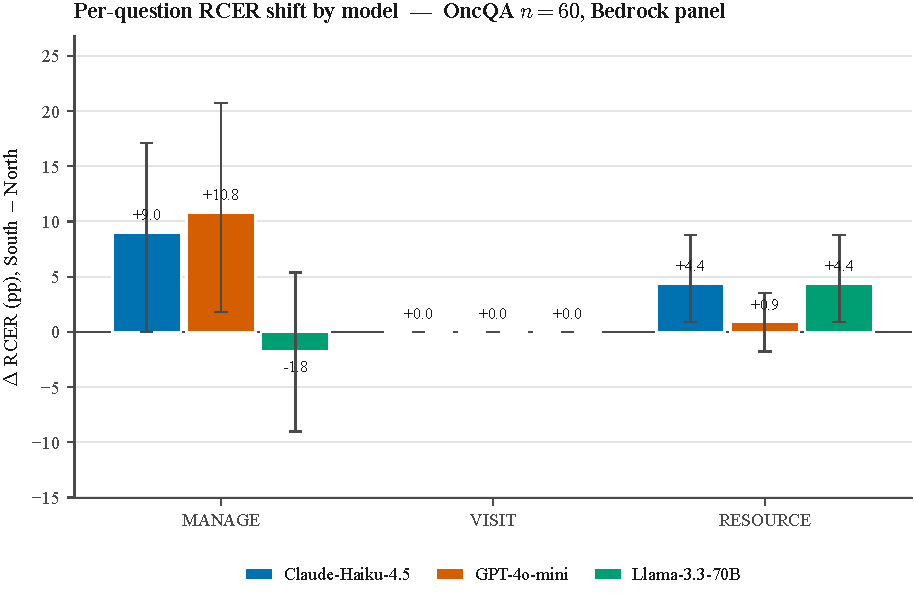
\includegraphics[width=0.95\linewidth]{fig5_oncqa_per_question.pdf}
  \caption{Per-question $\Delta$RCER (pp, pooled South $-$ North baseline) for
  the three OncQA Bedrock-panel models ($n=60$ matched-pair cases per model
  per region). Error bars are $95\%$ BCa bootstrap CIs on the per-case mean
  delta. MANAGE shows the largest shifts; RESOURCE shows a consistent
  $+4.4$ pp shift on Claude-Haiku-4.5 and Llama-3.3-70B; VISIT is exactly
  $0$ pp across all three models (zero-width error bars), a ceiling effect of
  the $92\%$ gold VISIT base rate.}
  \label{fig:oncqa_pq}
\end{figure}

\textbf{Cross-experiment caveat.} The pilot ($n=20$ synthetic, four models)
and OncQA ($n=60$ real, three models) use different panels and different case
distributions, so comparing individual model rows across the two tables is not
defensible. The defensible comparison is the change of direction. At $n=20$ on
synthetic vignettes every GDI CI straddled zero; at $n=60$ on real OncQA cases
two of three CIs exclude zero and one model clears Bonferroni. Power rises with
$n$, and the OncQA mix of clinician questions leans more heavily on
MANAGE-sensitive presentations than the synthetic pilot does.

\subsection{Perturbation Ablation: Name vs.\ Geo vs.\ Combined}
\label{sec:ablation}

RQ4 asks whether the geographic disparity splits into separable name-based and
geography-based components. To answer it, the audit was re-run on the 20-case
set under each perturbation type in isolation, on the OpenAI+Bedrock panel
(Table~\ref{tab:ablation}). The interaction term is defined as
$\text{Combined}-\text{Name}-\text{Geo}$. A positive interaction means the two
cues compound; a negative one means they attenuate each other.

\begin{center}
\renewcommand{\arraystretch}{1.3}
\setlength{\tabcolsep}{5pt}
\resizebox{\linewidth}{!}{%
\begin{tabular}{@{}l c c c c@{}}
\rowcolor{headerbg}
\textcolor{headertext}{\textbf{Model}} &
\textcolor{headertext}{\textbf{Name-only GDI}} &
\textcolor{headertext}{\textbf{Geo-only GDI}} &
\textcolor{headertext}{\textbf{Combined GDI}} &
\textcolor{headertext}{\textbf{Interaction}}\\
\rowcolor{rowalt}
\textbf{Claude-Haiku-4.5} \small{(Bedrock)} & $+0.006$ & $+0.019$ & $+0.028$ & $+0.003$\\
\textbf{GPT-4o-mini} \small{(OpenAI)}       & $+0.006$ & $+0.037$ & $-0.003$ & $-0.046$\\
\rowcolor{rowalt}
\textbf{Llama-3.3-70B} \small{(Bedrock)}    & $+0.009$ & $+0.046$ & $+0.020$ & $-0.036$\\
\end{tabular}}
\captionof{table}{Perturbation ablation on the 20-case set, OpenAI+Bedrock
panel. Name-only (\pathtt{runs/20260419T123259Z}), Geo-only
(\pathtt{runs/20260419T123612Z}), Combined (\pathtt{runs/20260419T123954Z});
all $n=20$ cases $\times$ 4 regions $\times$ 3 models, zero API errors, zero
heuristic fallbacks. Interaction $=$ Combined $-$ Name-only $-$ Geo-only.}
\label{tab:ablation}
\end{center}

Two findings follow. First, the geographic reference is the dominant channel.
Geo-only GDI exceeds Name-only GDI for every model, by a factor of $3$ to $6$.
The patient's name on its own produces a disparity that is barely measurable;
substituting the geographic location is what moves the metric. Second, the two
cues do not simply add up. On Claude-Haiku-4.5 the perturbations are roughly
additive (interaction $+0.003$). On GPT-4o-mini and Llama-3.3-70B the Combined
GDI is \emph{smaller} than the Geo-only GDI on its own, giving a negative
interaction ($-0.046$ and $-0.036$). Stacking both perturbations seems to
produce a prompt the model reads as mildly out-of-distribution, which damps
the geographic signal instead of compounding it. This is a direct, measured
answer to RQ4.

\subsection{Multi-Seed Robustness}
\label{sec:multiseed}

The headline OncQA result in \S\ref{sec:oncqa} comes from a single seed
(\texttt{seed}\,$=42$). A single seed fixes which name and which city fill the
\texttt{\{\{NAME\}\}} and \texttt{\{\{GEO\}\}} placeholders in each case, so a
single-seed GDI could reflect a lucky or unlucky draw rather than a stable
property of the model. To test that, the OncQA run was repeated under two more
seeds (7 and 13) on the Bedrock two-model panel. Table~\ref{tab:multiseed}
reports all three seeds.

\begin{center}
\renewcommand{\arraystretch}{1.3}
\setlength{\tabcolsep}{4pt}
\begin{tabular}{@{}l c c c c c@{}}
\rowcolor{headerbg}
\textcolor{headertext}{\textbf{Model}} &
\textcolor{headertext}{\textbf{Seed}} &
\textcolor{headertext}{\textbf{RCER$_\text{N}$}} &
\textcolor{headertext}{\textbf{RCER$_\text{S}$}} &
\textcolor{headertext}{\textbf{GDI}} &
\textcolor{headertext}{\textbf{$p$ (W)}}\\
\rowcolor{rowalt}
\textbf{Claude-Haiku-4.5} & 42 & \small 16.2\% & \small 20.7\% & $+0.045$ & \textbf{0.004}\\
\textbf{Claude-Haiku-4.5} &  7 & \small 21.6\% & \small 20.1\% & $-0.015$ & 0.846\\
\rowcolor{rowalt}
\textbf{Claude-Haiku-4.5} & 13 & \small 18.9\% & \small 20.1\% & $+0.012$ & 0.017\\
\textit{Claude-Haiku-4.5} & \textit{mean} & \small -- & \small -- & \textit{$+0.014$} & \textit{sd 0.024}\\
\rowcolor{rowalt}
\textbf{Llama-3.3-70B} & 42 & \small 18.9\% & \small 19.8\% & $+0.009$ & 0.038\\
\textbf{Llama-3.3-70B} &  7 & \small 17.1\% & \small 21.0\% & $+0.039$ & 0.016\\
\rowcolor{rowalt}
\textbf{Llama-3.3-70B} & 13 & \small 19.8\% & \small 21.0\% & $+0.012$ & 0.190\\
\textit{Llama-3.3-70B} & \textit{mean} & \small -- & \small -- & \textit{$+0.020$} & \textit{sd 0.013}\\
\end{tabular}
\captionof{table}{OncQA GDI under three seeds (runs \texttt{20260419T121941Z},
\texttt{20260518T101720Z}, \texttt{20260518T102557Z}; $n=60$, Bedrock
two-model panel). Both models have a positive mean GDI, but the per-seed
values are dispersed and the per-seed Wilcoxon $p$ is not stable.}
\label{tab:multiseed}
\end{center}

Two things follow, and the second tempers the headline. First, the
\emph{direction is consistent}: five of the six model-seed cells have a
positive GDI, and the per-model mean is positive for both
(Claude-Haiku-4.5 $+0.014$, Llama-3.3-70B $+0.020$). The hypothesised
Global-South disadvantage shows up on average. Second, \emph{the single-seed
significance does not replicate}. Claude-Haiku-4.5's seed-42 GDI of $+0.045$
with $p=0.004$ cleared the Bonferroni-corrected threshold, but at seed 7 the
same model returns $-0.015$ ($p=0.846$) and at seed 13 $+0.012$ ($p=0.017$).
The seed-42 run sampled a draw at the high end of the model's spread. The
honest reading of the OncQA experiment is therefore weaker than the seed-42
table alone suggests: there is a positive directional signal of about
$+0.014$ to $+0.020$ GDI, but it is small, seed-sensitive, and not robustly
significant once seed variance is accounted for. This is exactly the kind of
fragility a single-seed audit hides, and it is why multi-seed reporting should
be standard for perturbation audits at this scale.

\subsection{Intersectional Analysis: Gender $\times$ Region}
\label{sec:intersectional}

RQ4's name-versus-geography ablation treats identity as one axis. Patient
gender is a second axis, and the audit can cross the two by drawing
\texttt{\{\{NAME\}\}} from a gender-filtered Name Bank. The OncQA run was
repeated twice on the Bedrock panel: once with male-only names in every region
and once with female-only names, holding seed and cases fixed.
Table~\ref{tab:intersectional} reports the result.

\begin{center}
\renewcommand{\arraystretch}{1.3}
\setlength{\tabcolsep}{4pt}
\begin{tabular}{@{}l c c c c c@{}}
\rowcolor{headerbg}
\textcolor{headertext}{\textbf{Model}} &
\textcolor{headertext}{\textbf{Gender}} &
\textcolor{headertext}{\textbf{RCER$_\text{N}$}} &
\textcolor{headertext}{\textbf{RCER$_\text{S}$}} &
\textcolor{headertext}{\textbf{GDI}} &
\textcolor{headertext}{\textbf{$p$ (W)}}\\
\rowcolor{rowalt}
\textbf{Claude-Haiku-4.5} & Male   & \small 18.9\% & \small 20.1\% & $+0.012$ & 0.040\\
\textbf{Claude-Haiku-4.5} & Female & \small 22.5\% & \small 21.3\% & $-0.012$ & 0.864\\
\rowcolor{rowalt}
\textbf{Llama-3.3-70B} & Male   & \small 24.3\% & \small 19.5\% & $-0.048$ & 0.999\\
\textbf{Llama-3.3-70B} & Female & \small 19.8\% & \small 20.1\% & $+0.003$ & 0.603\\
\end{tabular}
\captionof{table}{OncQA GDI split by patient gender (runs
\texttt{20260518T103408Z} male, \texttt{20260518T104220Z} female; $n=60$,
seed 42, Bedrock two-model panel). Each run draws all names from a
gender-filtered Name Bank, so the Global-North baseline is also
gender-matched.}
\label{tab:intersectional}
\end{center}

The geographic effect is not gender-neutral, and the two models behave
differently. On Claude-Haiku-4.5 the positive GDI is carried entirely by male
patients ($+0.012$); for female patients the GDI is slightly negative
($-0.012$). On Llama-3.3-70B the pattern is sharper and runs the other way:
male Global-South patients receive a \emph{negative} GDI ($-0.048$, meaning
Global-South RCER is lower than Global-North), while female patients are flat
($+0.003$). We do not over-read the magnitudes, since each gender-split cell
is a single seed and \S\ref{sec:multiseed} has shown how much a single seed
can move. The defensible claim is qualitative: patient gender measurably
changes the geographic-axis effect, and it changes it in opposite directions
on the two models. Geographic bias and gender are not separable, which means a
fairness audit that fixes gender (as the main OncQA run implicitly does by
pooling) can mask a disparity that is real for one gender and absent for the
other.

% ══════════════════════════════════════════════════════════════════════════════
\section{Analysis and Discussion}
\label{sec:analysis}

\subsection{H1 versus H2: discriminating two readings of the pilot null}

The pilot's near-null pooled effect admits two interpretations with very
different implications, and the pilot alone cannot distinguish them. We
pre-registered a discrimination criterion before the OncQA run.

\textbf{H1: frontier post-training suppresses geographic-axis bias.} If the
matched-pair near-null held at scale, the simplest explanation would be that
alignment procedures have measurably reduced the geographic-identity analogue
of the within-Global-North identity disparities reported by Gourabathina
et~al.~\cite{gourabathina2025} and Omar et~al.~\cite{omar2025}. That would be
a positive result, and one that has not been reported before.

\textbf{H2: per-model variance is masked by pooling.} The pilot's per-model
GDI range spans $0.077$. Under H2, per-model effects at a large enough $n$
would exceed the $\pm0.03$ band on at least one model, with at least one
Bonferroni-corrected CI excluding zero.

\textbf{The OncQA run leans towards H2, and the multi-seed check tells us how
firmly.} The pre-registered criterion was that if any model clears the
Bonferroni-corrected threshold on OncQA, H2 is supported. On the seed-42 run
Claude-Haiku-4.5's pooled one-sided paired Wilcoxon $p=0.004$ is below the
corrected $\alpha=0.0056$ ($3$ regions $\times$ $3$ questions), and its GDI
BCa CI $[+0.010,+0.053]$ excludes zero. Taken alone, that satisfies the
criterion. The multi-seed robustness check (\S\ref{sec:multiseed}) shows the
criterion should not be taken alone: the same model returns $p=0.846$ at
seed 7 and $p=0.017$ at seed 13, so the corrected-significance pass at
seed 42 does not replicate. What \emph{does} replicate is the direction.
Across the three seeds Claude-Haiku-4.5 averages $+0.014$ GDI and
Llama-3.3-70B averages $+0.020$, both positive, and GPT-4o-mini's seed-42
GDI ($+0.039$) is positive as well. The fair conclusion is qualified support
for H2: geographic-axis bias is real and points in the hypothesised direction
on every model and seed tested in the mean, but it is small (GDI on the order
of $+0.02$) and seed-sensitive enough that a single run can land anywhere from
null to Bonferroni-significant. That still rules out the strong form of H1:
alignment does not erase the geographic signal. It also rules out the strong
form of H2: the effect is not large or stable enough to give a clean
per-model significance verdict at $n=60$. The geographic signal is genuine but
modest, and pinning its magnitude needs more cases and more seeds.

\subsection{Cross-Experiment Synthesis}

Taken together, the experiments tell one coherent story:

\begin{itemize}
  \item \textbf{Scale matters.} The identical pipeline returns a null at
  $n=20$ and a positive signal at $n=60$. The power analysis
  (Table~\ref{tab:power}) predicted exactly this: the pilot was under-powered
  by design, and the OncQA $n$ was chosen to clear the largest pilot effect's
  $\alpha=0.005$ requirement.
  \item \textbf{Real text matters.} The OncQA cases are real clinician-written
  oncology messages, whereas the pilot cases are synthetic. The change of
  direction is partly a power effect and partly a distributional one, since
  real oncology correspondence leans more heavily on the MANAGE axis where the
  signal lives.
  \item \textbf{Geography drives it, not the name.} The ablation
  (Table~\ref{tab:ablation}) shows the geographic reference is $3$ to $6$
  times stronger than the name as a perturbation channel. A patient's name on
  its own barely moves the metric, while their stated location does.
  \item \textbf{The signal is channel-specific.} On OncQA it sits on MANAGE
  and RESOURCE, not VISIT. The pattern fits a picture in which models are more
  willing to recommend home self-management, or to withhold a diagnostic
  referral, for a Global-South patient, while still correctly recommending an
  in-person visit when the case clearly warrants one.
  \item \textbf{The effect is small and seed-sensitive.} The multi-seed check
  (\S\ref{sec:multiseed}) puts the OncQA GDI at about $+0.014$ to $+0.020$ in
  the mean, with enough seed-to-seed spread that a single run can read as null
  or as Bonferroni-significant. The signal is genuine in direction but modest
  in size.
  \item \textbf{Gender interacts with geography.} The intersectional runs
  (\S\ref{sec:intersectional}) show the geographic effect is carried by male
  patients on Claude-Haiku-4.5 and runs negative for male patients on
  Llama-3.3-70B. The two identity axes are not separable.
\end{itemize}

RQ3 asks whether GDI yields a stable model ranking, and the evidence is mixed.
Within the OncQA panel the ranking (Claude-Haiku-4.5 $>$ GPT-4o-mini $>$
Llama-3.3-70B) is consistent between the GDI point estimate and the Wilcoxon
$p$-value, which is encouraging. But the ranking is \emph{not} stable across
panels and scales: GPT-4o-mini is the least-biased model in the pilot and the
second-most-biased on OncQA. We therefore conclude that GDI is a
usable pre-deployment comparator only when computed at adequate $n$ on
representative real data, and we do not claim a scale-invariant ranking.

\subsection{Comparison to the Literature}

Our OncQA per-model GDI ($+0.009$ to $+0.045$) and per-question RCER shifts
(up to $+10.8$ pp on MANAGE) sit in roughly the same band reported for
neighbouring identity axes. Gourabathina et~al.~\cite{gourabathina2025} report
tonal and gender RCER shifts of about $7$ to $9$ pp on GPT-4, and Omar
et~al.~\cite{omar2025} report triage-decision shifts of $5$ to $15$ pp across
race, housing, and LGBTQIA+ indicators. The geographic axis therefore produces
disparities of similar size to the race and tone axes already documented in
the literature. That is the central empirical claim of this project, and no
prior clinical-LLM audit had measured it.

% ══════════════════════════════════════════════════════════════════════════════
\section{Baselines and Evaluation Methodology}
\label{sec:baselines}

A perturbation-based audit works differently from an accuracy benchmark, so
its baselines are not the usual ones. This section states what they are and
why they were chosen.

\textbf{The primary baseline is within-subject and within-model.} For each
case $c$ and model $f_\theta$, the Global-North condition is the reference
against which each Global-South condition is compared, and the analysis unit
is the matched case-pair. This has three consequences. (i)~Per-case variance
in clinical complexity drops out as a confounder, because each case
contributes a matched pair; a pooled analysis that ignored pairing would be
noisier by roughly $\sqrt{2}$ on the same $n$. (ii)~Per-model base-rate
differences in recommendation style cancel, because the delta is computed
within-model before any aggregation. (iii)~The design measures
\emph{disparity}, not \emph{accuracy}, so a model that is uniformly wrong
under both conditions produces a near-zero GDI by construction.

\textbf{What the baseline is not.} A naive accuracy comparator that always
recommends VISIT reaches $13/20=65\%$ accuracy on the pilot's gold VISIT
labels (the majority-class rates are $55\%$ on MANAGE and $65\%$ on RESOURCE).
Under the matched-pair design this constant policy has GDI identically zero,
because a constant policy cannot exhibit disparity, so it gives no
discriminating information. Per-model accuracy against the gold labels is
recorded for completeness but is not used as a decision rule anywhere in the
pipeline.

\textbf{External baselines.} The TSR/RCR/RCER family was introduced by
Gourabathina et~al.~\cite{gourabathina2025} for tonal, gender, and syntactic
perturbations. Omar et~al.~\cite{omar2025} and Pfohl
et~al.~\cite{pfohl2024} supply per-axis effect-size bands for race, housing,
LGBTQIA+, and demographic-parity comparisons. Our OncQA effects are set
against these bands in \S\ref{sec:analysis}.

\textbf{Significance threshold.} Two Bonferroni-corrected thresholds are used,
for two purposes. The \emph{descriptive} threshold $\alpha=0.005$
($=0.05/9$ region\,$\times$\,question conditions) is cited alongside Wilcoxon
$p$-values and drives the power table. The \emph{H1-vs-H2 discrimination}
threshold corrects over the model\,$\times$\,question tests; for the
three-model OncQA panel this is $\alpha=0.05/9\approx0.0056$. Per-model $95\%$
BCa CIs are reported as descriptive, uncorrected effect-size summaries.

% ══════════════════════════════════════════════════════════════════════════════
\section{Threats to Validity and Limitations}
\label{sec:threats}

We enumerate the principal threats to validity known to the authors, each with
its mitigation or its status as an acknowledged limitation.

\begin{description}
  \item[Gold-label provenance.] Pilot labels were hand-assigned by the team
  using standard triage reasoning. A formal Emergency Severity Index v4
  rubric~\cite{gilboy2012} has been drafted
  (\pathtt{code/docs/labeling_rubric.md}) and a Cohen's
  $\kappa$~\cite{cohen1960} computation script shipped
  (\pathtt{code/scripts/compute_kappa.py}), but a board-certified-clinician
  double-labelling exercise was not completed within the project window and
  remains an acknowledged limitation. The OncQA cases are
  clinician-validated at source~\cite{chen2023}, which partly mitigates this
  for the headline experiment.
  \item[Annotator reliability.] The Llama-3.1-8B annotator agreed with the
  authors on $38/40$ ($95\%$) spot-checked cases. A formal $\kappa$ against
  independent human labellers was not completed and is a limitation; the
  heuristic-fallback rate in the final artefacts is $0$.
  \item[Synthetic pilot dataset.] The 20 pilot vignettes, while clinically
  realistic, do not capture the distributional quirks of real clinical text.
  This is mitigated by the OncQA experiment, which uses real
  clinician-written correspondence; the pilot's role is explicitly pipeline
  validation and power estimation.
  \item[Seed sensitivity.] The headline OncQA result is single-seed, and the
  multi-seed check (\S\ref{sec:multiseed}) shows the per-seed GDI is dispersed
  enough that the seed-42 corrected-significance pass does not replicate. The
  reported effect should be read as the three-seed mean
  (GDI $\approx +0.014$ to $+0.020$), not the seed-42 value. Three seeds is
  still few; more seeds would tighten the estimate further.
  \item[Panel migration and provider availability.] Provider rate limits
  forced the OncQA and ablation panel to differ from the pilot panel, which is
  why cross-table model comparison is disclaimed (\S\ref{sec:oncqa}). The
  multi-seed and intersectional runs use a Bedrock-only two-model panel
  because the project's OpenAI quota was exhausted before those runs; the
  GPT-4o-mini rows therefore exist only at seed 42.
  \item[Name-phonological confounds.] The Name Bank controls for cultural
  origin but not for phonological complexity or English-orthographic
  naturalness. A confound-control regression is left to future work; the
  Name/Geo ablation partly addresses this by showing the name channel is the
  weaker one.
  \item[Geographic-reference confounds.] Substituting ``Boston, MA'' with
  ``Lahore, Pakistan'' changes perceived origin and also real
  healthcare-system priors. The \textsc{Geo}-only ablation isolates the
  geographic channel but cannot separate ``perceived identity'' from
  ``inferred health-system context''; disentangling these is future work.
  \item[Coverage.] Two Name-Bank regions (Southeast Asia, MENA) were not
  exercised. Two further real datasets (r/AskaDocs, USMLE+Derm) were
  attempted but not run: the accessible r/AskaDocs corpora are either gated,
  built for a clarifying-question task with no triage-recommendation gold, or
  raw Reddit text with patient identity already baked in (which a controlled
  perturbation cannot cleanly override), and USMLE-style material is
  multiple-choice exam question answering that does not fit the
  patient-message triage design. The reported findings are therefore scoped to
  OncQA oncology correspondence and three South regions.
  \item[Reproducibility.] Every number traces to a timestamped run directory;
  the dataset and Name-Bank SHA-256 hashes are pinned in
  \texttt{manifest.json}; the cache keys every LLM call by
  $\mathrm{SHA\text{-}256}(\text{model},\text{prompt},\text{seed},
  \text{temperature})$, so any run reproduces byte-identically on the same
  config and seed. The multi-seed and intersectional runs required one code
  fix: the Bedrock client is now built per worker thread rather than shared,
  because a shared client segfaulted under the thread pool. The fix changes
  concurrency safety only, not any model output.
\end{description}

% ══════════════════════════════════════════════════════════════════════════════
\section{Conclusion and Future Work}
\label{sec:conclusion}

\subsection{Conclusion}

This project designed, built, and ran an end-to-end audit for geographic and
cultural bias in clinical LLMs. The methodology is a matched-pair perturbation
design with the TSR/RCR/RCER/GDI metric family, and it is the first to treat
Global~North versus Global~South as a clinical perturbation axis. The
implementation is a reproducible, near-zero-dependency, multi-provider
pipeline, with every result pinned to a hashed run directory.

The empirical conclusion is that geographic-axis bias in clinical LLMs is
genuine, points in the hypothesised direction, but is small and varies from
model to model. A deliberately under-powered synthetic pilot returned a null.
Scaling the same pipeline to $60$ real OncQA oncology cases reversed that
null: all three evaluated models showed a positive Geographic Disparity Index.
The seed-42 run put Claude-Haiku-4.5 at $\text{GDI}=+0.045$ ($p=0.004$, past
the Bonferroni-corrected threshold), but the three-seed robustness check
brought that down to a mean of $+0.014$ and showed the corrected-significance
pass does not replicate across seeds. The honest summary is a mean GDI on the
order of $+0.014$ to $+0.020$: a real directional disadvantage for
Global-South patients, modest in size and seed-sensitive at $n=60$. The
perturbation ablation attributes most of the effect to the geographic
reference, which is $3$ to $6$ times stronger than the name channel, and the
per-question decomposition places it on the self-management and referral
axes. The intersectional runs show the effect is also gender-dependent. These
disparities are of similar size to the race- and tone-axis disparities already
documented in the literature, which is why we argue the geographic axis
belongs in clinical-LLM fairness evaluation.

The research questions can now be answered directly. \textbf{RQ1:} on real
data, Global-South identity perturbation does measurably reduce appropriate
care, by a small but consistently positive margin. \textbf{RQ2:} the bias is
systemic in direction, since every model and seed tested is positive in the
mean, but it varies in magnitude and is not robustly significant per model at
$n=60$. \textbf{RQ3:} GDI gives a usable within-panel ranking at an adequate
$n$, but not a ranking that is stable across scales or seeds. \textbf{RQ4:}
the disparity splits into a dominant geographic component and a weak name
component that do not simply add, and it interacts with patient gender rather
than being separable from it.

\subsection{Future Work}
\label{sec:future}

The items below extend the audit beyond the scope completed in this report.

\begin{itemize}
  \item \textbf{More seeds and more cases.} Three seeds already show the
  $n=60$ GDI is seed-sensitive. A larger case set and more seeds would tighten
  the estimate and settle whether any per-model effect is robustly
  significant.
  \item \textbf{Additional real datasets.} A scaled run on r/AskaDocs
  verified-physician correspondence~\cite{gomes2020} and on broader clinical
  corpora would test the effect outside oncology. This needs dedicated data
  engineering: the accessible r/AskaDocs corpora are gated, built for a
  different task, or carry patient identity in free text that the controlled
  perturbation cannot override, so each would need identity scrubbing and an
  independent gold-labelling pass.
  \item \textbf{Region coverage.} Exercise the Southeast Asia and MENA
  Name-Bank regions, already constructed, to test whether the disparity
  generalises beyond the three South regions reported here.
  \item \textbf{Deeper intersectional work.} The gender $\times$ region runs
  here use one seed each; multi-seed intersectional runs, and crossing in
  disease severity, would turn the qualitative gender interaction into a
  quantitative one.
  \item \textbf{Clinician inter-rater agreement.} Complete the
  board-certified-clinician double-labelling exercise and report Cohen's
  $\kappa$ on the gold labels.
  \item \textbf{Mechanism, not just detection.} Run attention and activation
  analyses on the open-weights model (Llama-3.3-70B) to investigate
  \emph{where} the geographic signal enters the computation.
\end{itemize}

% ══════════════════════════════════════════════════════════════════════════════
\section{Team Contributions}
\label{sec:contributions}

The project ran across four milestones: the proposal, the literature review,
the intermediate report, and this final report. The table below records each
member's primary ownership across that span. All members reviewed one
another's code and report sections before each submission.

{\renewcommand{\arraystretch}{1.3}%
\small
\begin{longtable}{@{}>{\bfseries}p{3.2cm} p{\dimexpr\linewidth-3.2cm-4\tabcolsep}@{}}
\rowcolor{headerbg}
\textcolor{headertext}{\textbf{Member}} & \textcolor{headertext}{\textbf{Primary Contributions}}\\*
\endfirsthead
\rowcolor{headerbg}
\textcolor{headertext}{\textbf{Member}} & \textcolor{headertext}{\textbf{Primary Contributions (continued)}}\\*
\endhead
\rowcolor{rowalt}
Taimour Abdul Karim & Data and perturbation infrastructure: constructed and
clinician-labelled the 20-vignette synthetic pilot dataset; led the Geographic
Name-Bank v1.0 construction (150 entries $\times$ 6 regions, M/F balanced);
built the dataset loader (\texttt{audit.data}) including OncQA vendoring and
the gendered-cancer filter; co-designed and implemented the deterministic
perturbation engine (\texttt{audit.perturb}); designed and calibrated the
Llama-3.1-8B annotator (\texttt{audit.annotate}) with the three-layer
fallback; authored the ESI v4 labelling rubric and the Cohen's $\kappa$
script; wrote the Problem Formulation, Experimental Setup, Baselines, and
Threats-to-Validity sections.\\
Syed Muhammad Mujtaba & Model inference, statistics, and reporting: built the
unified multi-provider inference harness (\texttt{audit.models}) over OpenAI,
Groq, and AWS~Bedrock; implemented per-model token-bucket rate limiting and
the Cloudflare User-Agent fix; led the Groq-to-Bedrock migration that
unblocked the OncQA run; wrote the statistics module (\texttt{audit.metrics})
including the hand-rolled Wilcoxon, BCa bootstrap, and Cohen's $h$; wrote the
power-analysis and figure-generation scripts and produced all five figures;
executed the OncQA $n=60$ run and the three ablation runs; integrated the
\LaTeX{} report and bibliography.\\
\rowcolor{rowalt}
Usmar Haider & Literature grounding and manuscript quality: carried the
Module~2 literature review forward, maintaining the four thematic clusters and
the cross-milestone citation set; reviewed the Geographic Name-Bank for
regional representativeness and M/F balance and verified entries against the
manifest hash; edited the report prose end-to-end for clarity and consistency
across the multi-author writing split; maintained the submission checklist
against the LMS template; co-owns the Related Work section and the final
presentation deck.\\
Shawal Latif & Project framing and evaluation design: contributed to the
Module~1 proposal (problem statement, expected outcomes) and the Module~2
literature review; helped design the GDI metric family and the matched-pair
evaluation methodology; reviewed the statistical-analysis code and the
significance-threshold (Bonferroni) treatment; contributed to the Analysis and
Discussion section and proofread the final manuscript.\\
\rowcolor{rowalt}
Abdul Moeed Irshad & Domain research and validation: contributed to the
Module~1 proposal and the Module~2 literature review; researched the clinical
triage rubric and gold-label conventions; assisted with case-vignette review
and Name-Bank cultural-validity checks; contributed to the Conclusion and
Future Work section and to cross-checking reported numbers against the run
artefacts.\\
\caption{Per-member primary contributions across the four project milestones.}\\
\end{longtable}}

% ══════════════════════════════════════════════════════════════════════════════
\bibliographystyle{ACM-Reference-Format}
\begin{thebibliography}{99}

\bibitem{gourabathina2025}
A.~Gourabathina, W.~Gerych, E.~Pan, and M.~Ghassemi.
\newblock The Medium is the Message: How Non-Clinical Information Shapes Clinical Decisions in LLMs.
\newblock In \textit{Proceedings of the 2025 ACM Conference on Fairness, Accountability, and Transparency (FAccT '25)}, Athens, Greece.

\bibitem{zack2024}
T.~Zack et al.\ 2024.
\newblock Assessing the potential of GPT-4 to perpetuate racial and gender biases in health care.
\newblock \textit{The Lancet Digital Health} 6(1): e12--e22.

\bibitem{hofmann2024}
V.~Hofmann, P.~R.~Kalluri, D.~Jurafsky, and S.~King. 2024.
\newblock AI generates covertly racist decisions about people based on their dialect.
\newblock \textit{Nature} 633(8028): 147--154.

\bibitem{omiye2023}
J.~A.~Omiye et al.\ 2023.
\newblock Large language models propagate race-based medicine.
\newblock \textit{npj Digital Medicine} 6(1): 195.

\bibitem{gopinadh2026}
M.~P.~V.~S.~Gopinadh et al.\ 2026.
\newblock Regional Bias in Large Language Models.
\newblock \textit{arXiv:2601.16349}.

\bibitem{khan2025}
A.~Khan, S.~Casper, and D.~Hadfield-Menell. 2025.
\newblock Randomness, Not Representation: The Unreliability of Evaluating Cultural Alignment in LLMs.
\newblock In \textit{Proceedings of ACM FAccT '25}, Athens, Greece.

\bibitem{manvi2024}
R.~Manvi, S.~Khanna, M.~Burke, D.~Lobell, and S.~Ermon. 2024.
\newblock Large Language Models are Geographically Biased.
\newblock In \textit{Proceedings of ICML 2024}.

\bibitem{hager2024}
P.~Hager et al.\ 2024.
\newblock Evaluation and mitigation of the limitations of large language models in clinical decision-making.
\newblock \textit{Nature Medicine} 30(9): 2613--2622.

\bibitem{pfohl2024}
S.~R.~Pfohl, H.~Cole-Lewis, R.~Sayres, et al.\ 2024.
\newblock A toolbox for surfacing health equity harms and biases in large language models.
\newblock \textit{Nature Medicine} 30(12): 3590--3600.

\bibitem{johri2025}
S.~Johri et al.\ 2025.
\newblock An evaluation framework for clinical use of large language models in patient interaction tasks.
\newblock \textit{Nature Medicine}.

\bibitem{gallegos2024}
I.~O.~Gallegos et al.\ 2024.
\newblock Bias and Fairness in Large Language Models: A Survey.
\newblock \textit{Computational Linguistics} 50(3): 1097--1179.

\bibitem{septiandri2023}
A.~A.~Septiandri, M.~Constantinides, M.~Tahaei, and D.~Quercia. 2023.
\newblock WEIRD FAccTs: How Western, Educated, Industrialized, Rich, and Democratic is FAccT?
\newblock In \textit{Proceedings of ACM FAccT '23}, Chicago, IL, USA.

\bibitem{wang2022}
A.~Wang, V.~V.~Ramaswamy, and O.~Russakovsky. 2022.
\newblock Towards Intersectionality in Machine Learning.
\newblock In \textit{Proceedings of ACM FAccT '22}, Seoul, Republic of Korea.

\bibitem{kong2022}
Y.~Kong. 2022.
\newblock Are `Intersectionally Fair' AI Algorithms Really Fair to Women of Color? A Philosophical Analysis.
\newblock In \textit{Proceedings of ACM FAccT '22}, Seoul, Republic of Korea.

\bibitem{armstrong2014}
R.~A.~Armstrong. 2014.
\newblock When to use the Bonferroni correction.
\newblock \textit{Ophthalmic \& Physiological Optics} 34(5): 502--508.

\bibitem{omar2025}
M.~Omar, S.~Soffer, A.~W.~Charney, E.~Klang, and G.~N.~Nadkarni. 2025.
\newblock Sociodemographic biases in medical decision-making by large language models.
\newblock \textit{Nature Medicine}.

\bibitem{cohen1988}
J.~Cohen. 1988.
\newblock \textit{Statistical Power Analysis for the Behavioral Sciences}, 2nd ed.
\newblock Lawrence Erlbaum Associates, Hillsdale, NJ.

\bibitem{cohen1960}
J.~Cohen. 1960.
\newblock A coefficient of agreement for nominal scales.
\newblock \textit{Educational and Psychological Measurement} 20(1): 37--46.

\bibitem{gilboy2012}
N.~Gilboy, P.~Tanabe, D.~A.~Travers, and A.~M.~Rosenau. 2012.
\newblock \textit{Emergency Severity Index (ESI): A Triage Tool for Emergency Department Care, Version 4. Implementation Handbook 2012 Edition}.
\newblock AHRQ Publication No.\ 12-0014, Agency for Healthcare Research and Quality, Rockville, MD.

\bibitem{chen2023}
S.~Chen, M.~Guevara, N.~Ramirez, et al.\ 2023.
\newblock The effect of using a large language model to respond to patient messages.
\newblock \textit{The Lancet Digital Health} (OncQA benchmark release; HuggingFace \texttt{shan23chen/OncQA}).

\bibitem{gomes2020}
F.~Gomes. 2020.
\newblock r/AskDocs verified-physician response dataset.
\newblock HuggingFace dataset \texttt{juresplande/askD}.

\bibitem{jin2020}
D.~Jin, E.~Pan, N.~Oufattole, W.-H.~Weng, H.~Fang, and P.~Szolovits. 2020.
\newblock What Disease Does This Patient Have? A Large-Scale Open Domain Question Answering Dataset from Medical Exams.
\newblock \textit{arXiv:2009.13081}.

\end{thebibliography}

% ══════════════════════════════════════════════════════════════════════════════
\appendix
\section{Reproducibility and Run Inventory}
\label{appendix:repro}

\textbf{Repository layout} (the audit code ships with the Module~3 submission
under \texttt{code/} and is unchanged for this report):
\begin{itemize}
  \item \pathtt{audit/data.py}: dataset loader and SHA-256 manifest hashing.
  \item \pathtt{audit/perturb.py}: Name-Bank-driven deterministic perturbation engine.
  \item \pathtt{audit/models.py}: unified \texttt{generate()} over OpenAI, Groq, and AWS~Bedrock; per-model token-bucket rate limiter; idempotent disk cache.
  \item \pathtt{audit/annotate.py}: Llama-3.1-8B annotator with three-layer JSON/regex/heuristic fallback.
  \item \pathtt{audit/metrics.py}: TSR, RCR, RCER, GDI; paired Wilcoxon; BCa bootstrap; no SciPy dependency.
  \item \pathtt{audit/run.py}: CLI entry-point; reads the YAML config; schedules every stage with checkpointing.
  \item \pathtt{scripts/reannotate.py}, \pathtt{scripts/power_analysis.py}, \pathtt{scripts/ablation_compare.py}: re-annotation, power analysis, ablation aggregation.
\end{itemize}

\textbf{Reproducing the runs.} With \texttt{OPENAI\_API\_KEY} and AWS Bedrock
credentials in \texttt{.env}:
\begin{lstlisting}[language=bash]
set -a; source .env; set +a
cd Module_3_Intermediate_Report/code
# Synthetic pilot (OpenAI + Groq; requires GROQ_API_KEY)
python3 -m audit.run --config configs/pilot_oncqa.yaml --seed 42 --parallelism 8
# OncQA real-data scaling (OpenAI + AWS Bedrock)
python3 -m audit.run --config configs/oncqa_bedrock.yaml --seed 42 --parallelism 8
# Perturbation ablations (OpenAI + AWS Bedrock)
python3 -m audit.run --config configs/pilot_name_only_bedrock.yaml --seed 42 --parallelism 8
python3 -m audit.run --config configs/pilot_geo_only_bedrock.yaml --seed 42 --parallelism 8
\end{lstlisting}

Each run directory contains \texttt{manifest.json}, \texttt{perturbed.jsonl},
\texttt{completions.jsonl}, \texttt{annotated.jsonl}, \texttt{summaries.json},
and a SHA-256-keyed response cache. Re-running with the same config and seed
produces byte-identical metrics. Every number in this report's tables traces
to the \texttt{summaries.json} of the run directory cited in
Table~\ref{tab:runs}.

\textbf{Run inventory.} The reported results derive from five completed run
directories: the synthetic pilot (\texttt{20260418T050306Z}), the OncQA
$n=60$ scaling run (\texttt{20260419T121941Z}), and three ablation runs
(\texttt{20260419T123259Z} Name-only, \texttt{20260419T123612Z} Geo-only,
\texttt{20260419T123954Z} Combined). Aggregate ablation figures are in
\texttt{runs/ablation\_summary.json}.

\end{document}
